\documentclass[journal=jctcce,manuscript=article]{achemso}

\usepackage{amsmath,amssymb,mathtools}
\usepackage{booktabs}
\usepackage{siunitx}
\usepackage{tikz}
\usepackage{orcidlink}

\title{Unified Atomic Synthons and BDPCS3 for Continuous Chemical Space Exploration}

\author{Vincenzo Barone\,\orcidlink{0000-0001-6420-4107}}
\affiliation[c]{INSTM, via G. Giusti 9, 50121 Firenze, Italy}
\email{vincebarone52@gmail.com}

\author{Federico Lazzari\,\orcidlink{0000-0003-4506-3200}}
\affiliation{Scuola Superiore Meridionale, Largo San Marcellino 10, 80138 Napoli (Italy)}

\keywords{atomic synthons, continuous atom typing, BDPCS3, force-field correction, chemical space, effective atomic number}

\begin{document}

\begin{abstract}
Recent advances in high-accuracy quantum chemistry and molecular spectroscopy have extended investigations well beyond the traditional small-molecule regime, highlighting a persistent methodological gap in the representation, interpretation, and validation of molecular structure, topology, and chemical identity for medium-sized systems. Addressing this gap requires not only improved electronic-structure models, but also chemically grounded, transferable representations of complex molecular environments.

Here we present a unified framework that consolidates synthon-based descriptors, topology-aware structural analysis, symmetry, and robust coordinate transformations into one coherent paradigm for molecular structure and chemical-space characterization. Atomic synthons are reformulated as continuous, chemically interpretable descriptors of local environments, with contributions associated with steric, electrostatic, delocalization, and strain effects. Their normalized combination defines an effective atomic number, providing a continuous generalization of atomic identity for atoms in molecules and enabling robust similarity analysis.

Within this framework, topology, synthons, and BDPCS3 bond-length corrections share a single continuous descriptor layer, while Pisa Composite Schemes (in particular PCS2 references combined with the LCB25 library in this study) provide the high-accuracy electronic-structure backbone. Designed for regimes where high-quality reference datasets are intrinsically compact, the resulting workflow offers a chemically transparent basis for structure preparation, computation, validation, and transferable exploration of medium-sized molecular systems.
\end{abstract}

\section{Introduction}
The development of transferable molecular models requires descriptors that are simultaneously chemically meaningful, geometrically robust, and numerically smooth. Traditional atom typing schemes are often based on discrete rules or templates, which can be highly effective in narrow chemical domains but may become brittle across broad and heterogeneous chemical spaces. In particular, abrupt class boundaries can hinder interpolation between related environments and complicate parameter transfer from well-sampled regions to less explored areas of molecular space.

Although the general paradigm is formulated in a fully general manner, particular attention is devoted in the present work to molecular systems composed of the elements that dominate the chemistry of life and functional molecular complexity, namely C, N, O, F, P, S, Cl, Br, and I. These elements define the chemical backbone of organic, bio--relevant, and functional molecules, giving rise to a rich variety of bonding patterns, delocalization regimes, stereochemical constraints, and noncovalent interactions. Focusing on this chemically essential subset does not limit the generality of the framework, but rather reflects the fact that medium--sized molecules built from these elements represent the most challenging and scientifically relevant regime for modern quantum chemistry and molecular spectroscopy.

In this chemically dense domain, the limitations of conventional methodologies become particularly evident. Discrete atom typing, heuristic definitions of internal coordinates, and validation strategies applied \emph{a posteriori} are often insufficient to ensure structural reliability and chemical interpretability. These shortcomings motivate the development of continuous chemical descriptors, topology--aware representations, and non--redundant coordinate frameworks capable of capturing emergent molecular behavior beyond the small--molecule paradigm.

It is important to emphasize that the goal of the present work is not to compete with purely data--driven machine-learning approaches, nor to rely on extensive training datasets. In regimes dominated by high-accuracy quantum-chemical reference data, such datasets are necessarily limited in size, and the quality of the molecular representation becomes the decisive factor governing transferability and predictive power. The Merlin framework, as implemented here in Merlino 3.0, is explicitly designed for this regime, in which chemically informed descriptors act as compression operators that preserve relevant trends while enabling controlled interpolation from compact libraries of high-quality reference data.

Building on this motivation, we adopt \emph{continuous} local descriptors derived directly from geometry. In this work, we use atomic synthons as a compact continuous representation of the local environment. Synthons are designed to encode complementary information: pairwise bonding strength, local coordination, electron-domain structure, and geometric distortion. Because each component is continuous, synthons define a descriptor manifold where chemically related environments can be compared, clustered, and interpolated without imposing hard boundaries. At the formal level, this manifold is coupled to a weighted molecular graph in which continuous bond orders provide edge weights and synthons provide vertex attributes.

A second challenge is \emph{cross-module consistency}. In many practical workflows, topology analysis, descriptor construction, and geometry correction are implemented in separate modules with partially different definitions of coordination and bond order. Even small inconsistencies can propagate into nontrivial numerical drift: atoms may receive slightly different local characterizations depending on which module is queried, and correction models may respond to descriptor values that are not fully aligned with reporting and atom typing. Here we address this issue by enforcing a single continuous layer for coordination and bond-order quantities and by using that same layer in the BDPCS3 correction path.

From a methodological perspective, this unification supports three goals:
\begin{enumerate}
\item continuous atom typing for physically interpretable parameterization;
\item exploration and organization of chemical spaces through distance and similarity in descriptor space;
\item descriptor-driven correction of geometry and force-field quantities.
\end{enumerate}
In the present contribution, the first correction target is BDPCS3: only bond lengths are corrected from DPCS3, since angles and dihedrals are already sufficiently accurate in routine applications and therefore are kept unchanged at this stage.
The target accuracy is spectroscopic accuracy, i.e., the level required to reproduce equilibrium rotational constants within about 0.1\% for the parent isotopologue.

The same framework naturally extends beyond bond-length corrections. Once a coherent synthon space is available, equilibrium parameters, force constants, and cross terms can all be mapped to continuous functions of local descriptors, opening a path to transferable and differentiable force-field refinement strategies.

Within this framework, a key quantity is the effective atomic number, interpreted as a continuous molecular generalization of the isolated-atom atomic number:
\begin{equation}
Z^{\mathrm{eff}}_i = Z_i-\frac{1}{2}+\mathrm{ET}_i,
\end{equation}
where $\mathrm{ET}_i$ is an environmental tuning bounded in $[0,1)$. Defining
\begin{equation}
\mathbf{x}_i^{(\mathrm{ET})}=
\left(
\operatorname{erf}\!\left(\frac{q_i}{\sigma_{\mathrm{ET}}}\right),
\operatorname{erf}\!\left(\frac{C_i}{\sigma_{\mathrm{ET}}}\right),
\operatorname{erf}\!\left(\frac{D_i}{\sigma_{\mathrm{ET}}}\right),
\operatorname{erf}\!\left(\frac{S_i}{\sigma_{\mathrm{ET}}}\right)
\right),
\qquad
\mathrm{ET}_i=\frac{\lVert\mathbf{x}_i^{(\mathrm{ET})}\rVert_2}{1+\lVert\mathbf{x}_i^{(\mathrm{ET})}\rVert_2},
\end{equation}
$Z_i^{\mathrm{eff}}$ is explicitly the atomic number corrected by a normalized synthon norm (plus the constant shift $-0.5$). In this sense, $Z_i^{\mathrm{eff}}$ provides a bridge between symbolic chemistry (the integer $Z_i$) and continuous molecular embedding (the synthon norm).

The remainder of this paper is organized as follows. The Methods section introduces geometrical primitives, continuous coordination and bond-order definitions, and synthon construction, then details the coupling to BDPCS3. Results and Discussion focus on the implications of using one unified descriptor layer across topology, typing, and correction. The final section summarizes the methodological advantages and outlines extensions toward broader force-field correction tasks.

\section{Methods}
This section is organized from low-level geometry to high-level correction models. We first define continuous geometric and electronic descriptors, then assemble atomic and hierarchical synthons, and finally couple the resulting descriptor space to BDPCS3 bond-length corrections.

\subsection{Formal framework}
We represent a molecular structure as a weighted graph
\begin{equation}
G=(V,E,w),
\end{equation}
where vertices $v_i\in V$ are atoms, edges $(i,j)\in E$ are bonded interactions, and edge weights are given by continuous bond orders,
\begin{equation}
w_{ij}\equiv \mathrm{BO}_{ij}.
\end{equation}
This provides a continuous extension of classical molecular graphs, where topology and geometry are handled within one coherent layer.

Each atom is associated with an atomic synthon vector $\mathbf{s}_i\in\mathbb{R}^N$. Descriptor axes are treated as orthogonal basis vectors under the Euclidean inner product; this is a modeling assumption used to define a practical metric, not a claim of strict physical independence. Higher-order objects (bond, angle, dihedral, and ring synthons) are then constructed by composition over connected subgraphs, combining atomic synthons, bond orders, and geometric terms.
\subsection{Computational details}
All calculations and data processing were performed with the Merlino 3.0 workflow.
Implementation note: atomic synthons and BDPCS3 are available in two software contexts. Web implementations host legacy variants, including an approximate Cartesian-reconstruction strategy based on a genetic algorithm. Merlino implements the updated variants presented here, with Cartesian reconstruction performed through iterative internal-to-Cartesian updates based on the $\mathbf{B}$-matrix formalism.

\begin{table}[ht]
\caption{Implementation contexts for synthons and BDPCS3.}
\label{tab:impl_contexts}
\centering
\begin{tabular}{lll}
\toprule
Context & Model generation & Cartesian reconstruction \\
\midrule
Web tools (legacy) & Legacy synthons + legacy BDPCS3 & Approximate genetic-algorithm strategy \\
Merlino 3.0 (updated) & Updated synthons + updated BDPCS3 & Iterative $\mathbf{B}$-matrix internal-to-Cartesian update \\
\bottomrule
\end{tabular}
\end{table}

For full reproducibility, the following information is reported in the final submission:
\begin{enumerate}
\item electronic-structure level and basis set used to generate reference geometries (\textit{[PLACEHOLDER]});
\item optimizer and convergence thresholds (\textit{[PLACEHOLDER]});
\item topology/synthon module version and BDPCS3 implementation commit (\textit{[PLACEHOLDER]});
\item numerical tolerances used in internal-coordinate back-transformation (\textit{[PLACEHOLDER]}).
\end{enumerate}
Unless otherwise stated, distances are reported in \AA, rotational constants in MHz, and dimensionless descriptors are unitless.

\subsection{Computational cost and scalability}
The unified workflow is geometry-driven and dominated by repeated evaluations of pairwise distances and local descriptor terms. For a molecule with $N$ atoms, the descriptor layer scales approximately as $\mathcal{O}(N^2)$ for dense pair evaluations, while bonded and angle-level post-processing scales with graph sparsity in practical molecular systems. The BDPCS3 correction step itself is lightweight relative to upstream electronic-structure calculations and is therefore suitable for high-throughput post-processing.
The current implementation targets molecules up to about 100 atoms, where this $\mathcal{O}(N^2)$ regime is computationally adequate and robust in practice. For this reason, no linear-scaling machinery (e.g., neighbor-list/cell-list acceleration or sparse long-range screening) has been introduced yet. For substantially larger systems, dedicated linear- or near-linear-scaling strategies can be implemented without changing the underlying descriptor and correction formalism.

\subsection{Notation and symbols}
\begin{table}[ht]
\caption{Core notation and abbreviations used throughout the manuscript.}
\label{tab:notation}
\centering
\begin{tabular}{ll}
\toprule
Symbol & Meaning \\
\midrule
$R_{ij}$ & Interatomic distance between atoms $i$ and $j$ \\
$\theta_{ijk}$ & Bond angle centered on atom $i$ \\
$\mathrm{CNA}_i$ & Continuous coordination number \\
$\tilde R_i^{\mathrm{cov}}$ & Coordination-dependent effective covalent radius \\
$\mathrm{BO}_{ij}^{\mathrm{topo}}$ & Topology bond order \\
$N_{\mathrm{ED},i}$ & Number of electronic domains \\
$d_i$ & Topological degree ($|\mathcal{N}(i)|$) \\
$D_i^{\mathrm{dom}}$ & Domain-count symbol used in angular normalization ($D_i^{\mathrm{dom}}=N_{\mathrm{ED},i}$) \\
$q_i, C_i, D_i, S_i$ & Charge-like, covalency, radial-distortion, angular-strain descriptors \\
$\mathrm{ET}_i$ & Environmental Tuning (normalized synthon norm) \\
$Z_i^{\mathrm{eff}}$ & Effective atomic number \\
$D_B$ & Bhattacharyya distance between molecular Gaussian descriptor models \\
$\mathrm{Sim}=\exp(-D_B)$ & Synthon Gaussian similarity score \\
$D_B^{\mathrm{ring}}$, $\mathrm{Sim}_{\mathrm{ring}}$ & Ring-level Gaussian distance/similarity from cycle descriptors \\
$\mathrm{Sim}_{\mathrm{comb}}$ & Weighted combined similarity (synthon + ring term) \\
$\Delta r_{ij}$ & BDPCS3 bond-length correction \\
CNA, BO, ET & Continuous Coordination Number, Bond Order, Environmental Tuning \\
NED, NLP, NOS & Electronic domains, lone-pair count, unpaired-electron count \\
MAE, RMSE & Mean absolute error and root mean square error \\
\bottomrule
\end{tabular}
\end{table}

For clarity, when no superscript is shown, $\mathrm{BO}_{ij}$ refers to the topology-consistent bond order defined in Equation~\ref{eq:bo_topo}. This convention is used uniformly in descriptor and correction expressions.
All normalized or scaled descriptor quantities (e.g., CNA-, BO-, and synthon-derived dimensionless terms) are unitless by construction.

\begin{table}[ht]
\caption{Symbol reuse map: first definition points in the manuscript.}
\label{tab:symbol_reuse}
\centering
\begin{tabular}{ll}
\toprule
Symbol/group & First definition location \\
\midrule
$R_{ij}$, $\theta_{ijk}$ & Geometrical primitives \\
$\mathrm{CNA}_i$, $\tilde R_i^{\mathrm{cov}}$ & Continuous coordination and effective covalent radius \\
$\mathrm{BO}_{ij}$, $\mathrm{BO}^{(\pi)}_{ij}$ & Topological bond order \\
$N_{\mathrm{LP},i}$, $N_{\mathrm{OS},i}$, $N_{\mathrm{ED},i}$, $d_i$ & Electronic balance/domains and canonical identity \\
$q_i$, $C_i$, $D_i$, $S_i$, $\mathbf{x}_i$, $\mathbf{s}_i$ & Continuous descriptors and atomic synthons \\
$\mathrm{ET}_i$, $Z_i^{\mathrm{eff}}$ & Introduction (central concept) and synthons sections \\
$D_B$, $\mathrm{Sim}$ & Synthon Gaussian similarity subsection \\
$D_B^{\mathrm{ring}}$, $\mathrm{Sim}_{\mathrm{ring}}$, $\mathrm{Sim}_{\mathrm{comb}}$ & Ring-aware similarity subsection \\
$\Delta r_{ij}$, $K$, $\Delta r$, $\sigma$ & BDPCS3 coupling \\
\bottomrule
\end{tabular}
\end{table}

\subsection{Geometrical primitives}
Interatomic distances are
\begin{equation}
R_{ij}=\lVert\mathbf{r}_i-\mathbf{r}_j\rVert,
\end{equation}
and bond angles are
\begin{equation}
\theta_{ijk}=\angle(\mathbf{r}_j-\mathbf{r}_i,\mathbf{r}_k-\mathbf{r}_i).
\end{equation}

\subsection{Continuous coordination and effective covalent radius}
The continuous coordination number is
\begin{equation}
\mathrm{CNA}_i=\sum_{j\neq i} g_{ij},
\qquad
g_{ij}=\frac{1}{2}\left[1+\operatorname{erf}\!\left(\alpha_{\mathrm{CNA}}(R^0_{ij}-R_{ij})\right)\right],
\end{equation}
with
\begin{equation}
R^0_{ij}=R^{\mathrm{cov}}(Z_i)+R^{\mathrm{cov}}(Z_j).
\end{equation}

The coordination-dependent covalent radius is interpolated from tabulated Pyykko values:
\begin{equation}
\tilde R^{\mathrm{cov}}_i=\mathcal{H}(Z_i,\mathrm{CNA}_i),
\end{equation}
where $\mathcal{H}$ is a $C^1$ cubic Hermite interpolation.
This interpolation avoids discontinuities at integer coordination values and preserves smooth gradients required for geometry optimization and descriptor mapping.

\paragraph{Technical clarification retained from the original formulation.}
An equivalent smooth-coordination form can be written as
\begin{equation}
g(R_{ij})=
\frac{1}{2}\left[
1-\operatorname{erf}\!\left(
\frac{R_{ij}-R_{\mathrm{eff},ij}}
{\sigma_{\mathrm{CNA}}}
\right)\right],
\end{equation}
with
\begin{equation}
R_{\mathrm{eff},ij}=s\left(R_{\mathrm{cov},i}+R_{\mathrm{cov},j}\right),
\qquad s=\frac{4}{3}.
\end{equation}

\subsection{Topological bond order}
The bond order is
\begin{equation}
\mathrm{BO}_{ij}=\exp\!\left(\frac{\tilde R^{\mathrm{cov}}_i+\tilde R^{\mathrm{cov}}_j-R_{ij}}{\lambda_{\mathrm{BO}}}\right).
\label{eq:bo_topo}
\end{equation}
In the present implementation, $\lambda_{\mathrm{BO}}=0.20$ (dimensionless), corresponding to a Pauling-like decay length of approximately 0.30 \AA for a C--C reference bond.
The $\pi$ contribution is
\begin{equation}
\mathrm{BO}^{(\pi)}_{ij}=\max(\mathrm{BO}_{ij}-1,0).
\end{equation}

\subsection{Electronic balance and domains}
\begin{align}
N_{\pi,i} &= \sum_{j\in\mathcal{N}(i)} \mathrm{BO}^{(\pi)}_{ij},\\
N_{\mathrm{res},i} &= n^{\mathrm{val}}_i-\mathrm{CNA}_i-N_{\pi,i},\\
N_{\mathrm{OS},i} &= \mathrm{mod}(\mathrm{round}(N_{\mathrm{res},i}),2),\\
N_{\mathrm{LP},i} &= \max\!\left(0,\frac{N_{\mathrm{res},i}-N_{\mathrm{OS},i}}{2}\right),\\
N_{\mathrm{ED},i} &= \mathrm{CNA}_i+N_{\mathrm{LP},i}+N_{\mathrm{OS},i}.
\end{align}
The role of each term is as follows:
\begin{itemize}
\item $N_{\pi,i}$ measures the local $\pi$-bond excess beyond single-bond character and captures bond-strength redistribution in conjugated environments.
\item $N_{\mathrm{res},i}$ is the residual valence-electron balance after accounting for coordination and $\pi$ contribution.
\item $N_{\mathrm{OS},i}$ provides the odd-electron (open-shell) indicator derived from the parity of the rounded residual population.
\item $N_{\mathrm{LP},i}$ is the continuous lone-pair count, clipped at zero to avoid unphysical negative values.
\item $N_{\mathrm{ED},i}$ is the total electronic-domain count used downstream for geometry classification and reference-angle assignment.
\end{itemize}
This construction separates pairwise bond strengthening ($N_{\pi,i}$) from domain counting, yielding descriptors that are chemically interpretable and stable against small geometric perturbations.

\subsection{Angular strain}
Reference angular values are defined from an idealized domain geometry as a function of coordination.
For an integer coordination/domain number $N$, the mean reference angle is
\begin{equation}
\bar{\theta}(N)=\frac{\Theta(N)}{\binom{N}{2}},
\end{equation}
where $\Theta(N)$ is the total sum of ideal pair angles for that coordination shell.
For non-integer electronic-domain counts, a smooth cubic Hermite interpolation is used:
\begin{equation}
\theta^{\mathrm{ref}}(N^{\mathrm{dom}})=
h_{00}(t)\,\bar{\theta}(k)+
h_{10}(t)\,m_k+
h_{01}(t)\,\bar{\theta}(k+1)+
h_{11}(t)\,m_{k+1},
\end{equation}
with $k=\lfloor N^{\mathrm{dom}}\rfloor$ and $t=N^{\mathrm{dom}}-k$.
The lower bound is taken as $k_{\min}=2$ in the present coordination range.
The slopes are
\begin{equation}
m_k=
\begin{cases}
\bar{\theta}(k+1)-\bar{\theta}(k), & k=k_{\min},\\[4pt]
\dfrac{1}{2}\big[\bar{\theta}(k+1)-\bar{\theta}(k-1)\big], & \text{otherwise}.
\end{cases}
\end{equation}

\begin{table}[ht]
\caption{Reference angular sums and mean angles used for strain evaluation.}
\label{tab:ref_angles}
\centering
\begin{tabular}{cccc}
\toprule
Coordination & Geometry & Sum (deg) & Mean (deg) \\
\midrule
2  & Linear               & 180.0             & 180.0 \\
3  & Trigonal planar      & 360.0             & 120.0 \\
4  & Tetrahedral          & $6 \times 109.47$ & 109.47 \\
5  & Trigonal bipyramidal & 720.0             & 120.0 \\
6  & Octahedral           & $12 \times 90.0$  & 90.0  \\
7  & Capped octahedral    & 1260.0            & 120.0 \\
8  & Cubic                & $24 \times 90.0$  & 90.0  \\
12 & Icosahedral          & $30 \times 63.43$ & 63.43 \\
\bottomrule
\end{tabular}
\end{table}

Using a cosine-based metric with reference angle $\theta_i^{\mathrm{ref}}$, where $D_i^{\mathrm{dom}} \equiv N_{\mathrm{ED},i}$ denotes the local domain count used for angular normalization:
\begin{equation}
S_i=
\left[
\frac{1}{\binom{D_i^{\mathrm{dom}}}{2}}
\sum_{j<k}
\left(\cos\theta_{ijk}-\cos\theta_i^{\mathrm{ref}}\right)^2
\right]^{1/2}.
\end{equation}

For completeness, two retained alternative forms are
\begin{equation}
S_i^{(\theta)}=
\left[
\frac{1}{\binom{D_i^{\mathrm{dom}}}{2}}
\sum_{j<k}\left(\theta_{ijk}-\theta_i^{\mathrm{ref}}\right)^2
\right]^{1/2},
\end{equation}
and
\begin{equation}
S_i^{(\cos^2)}=
\left[
\frac{1}{\binom{D_i^{\mathrm{dom}}}{2}}
\sum_{j<k}\left(\cos^2\theta_{ijk}-\cos^2\theta_i^{\mathrm{ref}}\right)^2
\right]^{1/2}.
\end{equation}

\subsection{Continuous descriptors and atomic synthons}
In generic form, an environment-corrected descriptor can be written as
\begin{equation}
X_i=
X_i^{(0)}+\sum_j\frac{X_j^{(0)}-X_i^{(0)}}{(n_i+n_j)\,\mathrm{BO}_{ij}}.
\end{equation}

Descriptors used in the synthon layer include:
\begin{align}
q_i &= \sum_{j\in\mathcal{N}(i)}\frac{\chi_j-\chi_i}{(n_i+n_j)\,\max(\mathrm{BO}_{ij},\mathrm{BO}_{\min})},\\
C_i &= \frac{1}{|\mathcal{N}(i)|}\sum_{j\in\mathcal{N}(i)}
\frac{\tilde R^{\mathrm{cov}}_i+\tilde R^{\mathrm{cov}}_j}{R_{ij}+\tilde R^{\mathrm{cov}}_i+\tilde R^{\mathrm{cov}}_j},\\
D_i &= \frac{1}{|\mathcal{N}(i)|\,\bar R_i}\sum_{j\in\mathcal{N}(i)}|R_{ij}-\bar R_i|,
\quad
\bar R_i=\frac{1}{|\mathcal{N}(i)|}\sum_{j\in\mathcal{N}(i)}R_{ij}.
\end{align}
Here, $q_i$ captures an electronegativity-driven local charge-transfer tendency, $C_i$ measures local covalent compactness (larger values for shorter and stronger local contacts), and $D_i$ quantifies bond-length dispersion around the local average. Together with the angular term $S_i$, these descriptors separate electronic imbalance, bond-strength character, radial distortion, and angular distortion within one continuous representation. In this sense, the synthon map acts as a chemically informed low-dimensional embedding designed for interpolation from compact, high-accuracy reference datasets.

A compact continuous synthon is therefore represented by
\begin{equation}
\mathbf{x}_i=(q_i,\,C_i,\,D_i,\,S_i),
\end{equation}
with normalized magnitude $\mathrm{ET}_i$ given above.
In the present workflow, this four-component representation is the operational descriptor used for $\mathrm{ET}_i$, $Z_i^{\mathrm{eff}}$, descriptor-space distances, and BDPCS3-coupled analyses.

For compatibility with earlier developments and possible extensions (e.g., explicit delocalization/polarizability channels), the original five-component form is retained as
\begin{equation}
\mathbf{s}_i=(q_i,\,\alpha_i,\,C_i,\,S_i,\,D_i^{(\pi)}),
\end{equation}
where $D_i^{(\pi)}$ denotes the delocalization component and $\alpha_i$ the polarizability-like contribution.
Its intrinsic normalized norm can be expressed as
\begin{equation}
I_i=\frac{\lVert\mathbf{s}_i\rVert}{\lVert\mathbf{s}\rVert_{\max}}\in[0,1],
\end{equation}
which is consistent with the role played by $\mathrm{ET}_i$ in the present implementation.

The corresponding atom-synthon metric is
\begin{equation}
d_{ij}^{(\mathrm{atom})}=
\sqrt{
\left(Z_i^{\mathrm{eff}}-Z_j^{\mathrm{eff}}\right)^2+
\lVert\mathbf{x}_i-\mathbf{x}_j\rVert_2^2
}.
\end{equation}
When needed, an extended five-component distance can be defined analogously on $\mathbf{s}_i$.

\subsection{Gaussian similarity in synthon space}
For molecule-level comparison, atomic descriptors are aggregated as
\begin{equation}
X=
\begin{bmatrix}
\mathbf{x}_1^\mathsf{T}\\
\vdots\\
\mathbf{x}_N^\mathsf{T}
\end{bmatrix},
\qquad
\mathbf{x}_i=(q_i,\,C_i,\,D_i,\,S_i,\,Z_i^{\mathrm{eff}}),
\end{equation}
and fitted with a Gaussian model $(\boldsymbol{\mu},\mathbf{\Sigma})$:
\begin{equation}
\boldsymbol{\mu}=\frac{1}{N}\sum_{i=1}^{N}\mathbf{x}_i,
\qquad
\mathbf{\Sigma}=
\begin{cases}
\mathrm{Cov}(X)+\lambda\mathbf{I} & \text{(full)},\\
\mathrm{diag}(\mathrm{Cov}(X))+\lambda\mathbf{I} & \text{(diag)},
\end{cases}
\end{equation}
with regularization $\lambda>0$.

Given molecules $A$ and $B$, define
\begin{equation}
\Delta\boldsymbol{\mu}=\boldsymbol{\mu}_A-\boldsymbol{\mu}_B,
\qquad
\mathbf{\Sigma}=\frac{1}{2}\left(\mathbf{\Sigma}_A+\mathbf{\Sigma}_B\right).
\end{equation}
Their Bhattacharyya distance is
\begin{equation}
D_B=
\frac{1}{8}\Delta\boldsymbol{\mu}^\mathsf{T}\mathbf{\Sigma}^{-1}\Delta\boldsymbol{\mu}
+\frac{1}{2}\left[
\ln\det\mathbf{\Sigma}
-\frac{1}{2}\left(\ln\det\mathbf{\Sigma}_A+\ln\det\mathbf{\Sigma}_B\right)
\right],
\end{equation}
and the bounded similarity score is
\begin{equation}
\mathrm{Sim}(A,B)=\exp(-D_B)\in(0,1].
\end{equation}
To include explicit cycle comparison (positions and topology of rings), each detected ring is also embedded by
\begin{equation}
\mathbf{r}_k = \big(
\text{size},\ \text{planarity},\ \text{radial position},\ \text{fused degree},\ \text{nearest-centroid distance},\ \text{ring radius}
\big)_k,
\end{equation}
where radial/centroid quantities are normalized by a molecular size scale.
The same Gaussian/Bhattacharyya construction yields a ring score
\begin{equation}
\mathrm{Sim}_{\mathrm{ring}}(A,B)=\exp\!\left(-D_B^{\mathrm{ring}}\right).
\end{equation}
The final ranking metric is
\begin{equation}
\mathrm{Sim}_{\mathrm{comb}}(A,B)=
\left(1-w_{\mathrm{ring}}\right)\mathrm{Sim}(A,B)+w_{\mathrm{ring}}\mathrm{Sim}_{\mathrm{ring}}(A,B),
\end{equation}
with default $w_{\mathrm{ring}}=0.25$. If both molecules are acyclic, the ring term is disabled (effective $w_{\mathrm{ring}}=0$), so the score reduces to $\mathrm{Sim}(A,B)$.
This combined definition is used for pairwise reporting and query-vs-library ranking.

\subsection{Hierarchical synthons}
Bond, angle, and dihedral synthons are defined by composition of atomic descriptors and local geometry:
\begin{align}
\mathcal{S}^{(\mathrm{bond})}_{ij} &= (\mathbf{x}_i,\mathbf{x}_j,\mathrm{BO}_{ij}),\\
\mathcal{S}^{(\mathrm{angle})}_{ijk} &= (\mathbf{x}_i,\mathbf{x}_j,\mathbf{x}_k,\mathrm{BO}_{ij},\mathrm{BO}_{jk},\cos\theta_{ijk}),\\
\mathcal{S}^{(\mathrm{dihedral})}_{ijkl} &= (\mathcal{S}^{(\mathrm{bond})}_{ij},\mathcal{S}^{(\mathrm{bond})}_{jk},\mathcal{S}^{(\mathrm{bond})}_{kl},\cos\phi_{ijkl},\cos^2\phi_{ijkl}).
\end{align}
These hierarchical objects provide a natural bridge between local atom typing and higher-order force-field terms.

\subsection{Canonical atomic identity}
Each atom is represented at two complementary levels: a canonical discrete identity and a continuous synthon coordinate. The separation is strict: discrete quantities define identity classes, while continuous coordinates are used for similarity and interpolation.

In parallel to the continuous synthon space, a compact canonical signature is used:
\begin{equation}
\Sigma_i=(Z_i,\,\mathrm{aromatic}_i,\,\mathrm{round}(N_{\mathrm{ED},i}),\,d_i),
\end{equation}
with topological degree
\begin{equation}
d_i=|\mathcal{N}(i)|.
\end{equation}

\subsection{Ring detection and canonicalization}
Ring perception is performed on the discrete molecular graph using depth-first enumeration of simple cycles. A candidate cycle
\begin{equation}
C=(v_1,v_2,\dots,v_m)
\end{equation}
is accepted when all consecutive pairs (including $v_m\!-\!v_1$) are bonded and no vertex is repeated.
To remove duplicates generated by different traversal starts/directions, each cycle is mapped to a canonical representative
\begin{equation}
\mathrm{can}(C)=\min\Big(\{\rho_k(C)\}_{k=0}^{m-1}\cup\{\rho_k(C^{\mathrm{rev}})\}_{k=0}^{m-1}\Big),
\end{equation}
where $\rho_k$ denotes cyclic rotation and $C^{\mathrm{rev}}$ is reversed order. Canonical cycles are stored once and then used to build ring objects, atom--ring maps, bond--ring maps, and fused-ring connectivity.

The implementation supports an optional maximum ring size parameter ($\texttt{ring\_max}$). In the present Merlino workflow this cutoff is not enforced by default (full simple-cycle detection on the current graph), which is adequate for the target systems discussed here ($\sim$100 atoms). If needed for larger systems, $\texttt{ring\_max}$ can be activated to restrict ring enumeration to chemically relevant sizes.

\subsection{Point-group symmetry and equivalent parameters}
Merlino also provides automatic point-group assignment from the optimized Cartesian structure and uses the resulting symmetry operations to identify equivalent internal coordinates and equivalent force-field parameters.
The procedure is geometry-based and fully automated:
\begin{enumerate}
\item translate to the center of mass and rotate to principal-inertia axes;
\item generate candidate symmetry operations (proper/improper rotations, mirrors, inversion);
\item validate each operation by atom mapping under element-consistent distance tolerance;
\item classify the accepted operation set to assign the molecular point group.
\end{enumerate}
With centered Cartesian coordinates $\mathbf{r}_i$, the inertia tensor is
\begin{equation}
\mathbf{I}=\sum_i m_i\left[(\mathbf{r}_i\cdot\mathbf{r}_i)\mathbf{1}-\mathbf{r}_i\mathbf{r}_i^\mathsf{T}\right],
\end{equation}
and candidate operations are tested through $\mathbf{r}_i'=\mathbf{R}\mathbf{r}_i$ with atom matching constrained by
\begin{equation}
\left\lVert \mathbf{r}_i'-\mathbf{r}_{\pi(i)}\right\rVert < \tau,
\qquad
Z_{\pi(i)}=Z_i,
\end{equation}
where $\pi$ is the induced atom permutation and $\tau$ is the symmetry tolerance.

Equivalent geometric parameters are then obtained from the same permutation group action on primitive internals (bond stretches, valence angles, dihedrals, out-of-plane and linear-bend terms). Two geometric parameters are equivalent if they belong to the same symmetry orbit.
Given a molecular point group $G$, two primitives $p_a$ and $p_b$ are symmetry-equivalent when
\begin{equation}
\exists\, g\in G:\quad p_b=g\cdot p_a.
\end{equation}
This defines orbits (equivalence classes)
\begin{equation}
\mathcal{O}(p)=\{g\cdot p\;|\;g\in G\}.
\end{equation}
For any parameter family $\{k_p\}$ associated with primitives (bond, angle, dihedral terms), a symmetry-consistent representative can be written as
\begin{equation}
\bar{k}_{\mathcal{O}}=\frac{1}{|\mathcal{O}|}\sum_{p\in\mathcal{O}}k_p,
\end{equation}
and applied to all members of the same orbit. This reduces parameter redundancy, enforces exact equality of symmetry-equivalent terms, and improves robustness in descriptor-to-parameter mapping.
The same orbit construction is used in the GUI/report layer to list equivalent parameter classes by type (bond, angle, dihedral, out-of-plane, linear-bend).

\subsection{BDPCS3 coupling}
BDPCS3 corrections are applied to DPCS3 bond lengths using topology-consistent bond orders:
\begin{equation}
\mathrm{BO}_{ij}^{\mathrm{BDPCS3}} \leftarrow \mathrm{BO}_{ij}^{\mathrm{topo}}.
\end{equation}

Updated BDPCS3 equations are:
\begin{equation}
r_{ij}^{\mathrm{BDPCS3}}=r_{ij}^{\mathrm{DPCS3}}+\Delta r_{ij},
\end{equation}
\begin{equation}
\Delta r_{ij}=A_{ij}(r_{ij})\left[1-\chi_{\mathrm{CS}}(i)\chi_{\mathrm{CS}}(j)
\exp\!\left(-\left(\frac{r_{ij}-r^{\mathrm{cov}}_{ij}+\Delta r}{\sigma}\right)^2\right)\right],
\end{equation}
with
\begin{equation}
A_{ij}(r)=-K\,r^{\mathrm{cov}}_{ij}
\left(1+0.56\,\chi_{\mathrm{CH}}(i)\chi_{\mathrm{CH}}(j)\right)
\left[\max(n_i,n_j)^2-1\right]
f_{\mathrm{coord}}(r),
\end{equation}
\begin{equation}
f_{\mathrm{coord}}(r)=\frac{1}{2}\left[1-\operatorname{erf}\!\left(\frac{r-(r^{\mathrm{cov}}_{ij}+0.35)}{\sigma}\right)\right],
\end{equation}
\begin{align}
\chi_{\mathrm{CS}}(x)&=\delta_{Z_x,6}+0.5\,\delta_{Z_x,16},\\
\chi_{\mathrm{CH}}(x)&=\delta_{Z_x,6}+\delta_{Z_x,1}.
\end{align}
The selector $\chi_{\mathrm{CS}}$ activates the sulfur-specific modulation in C/S environments, while $\chi_{\mathrm{CH}}$ identifies C/H-containing pairs for the hydrocarbon-focused prefactor correction.

Parameters:
\begin{equation}
K=4.15\times10^{-4},\qquad
\Delta r=0.17~\text{\AA},\qquad
\sigma=0.057~\text{\AA}.
\end{equation}
These updated values are tuned to remain legacy-aligned within method precision (sub-m\AA level), while preserving full consistency with the unified topology-driven descriptor layer.

\paragraph{Implementation form.}
\begin{equation}
\Delta r_{ij}=
\left[-K\,r^{\mathrm{cov}}_{ij}(1+0.56\,\chi_{\mathrm{CH},ij})N_{ij}f_{\mathrm{coord}}(r)\right]
\left(1-\chi_{\mathrm{CS},ij}e^{-((r-r^{\mathrm{cov}}_{ij}+\Delta r)/\sigma)^2}\right),
\end{equation}
with $\chi_{\mathrm{CH},ij}=\chi_{\mathrm{CH}}(i)\chi_{\mathrm{CH}}(j)$,
$\chi_{\mathrm{CS},ij}=\chi_{\mathrm{CS}}(i)\chi_{\mathrm{CS}}(j)$,
$N_{ij}=\max(n_i,n_j)^2-1$.
Because all terms depend on the same continuous topology layer, BDPCS3 corrections remain aligned with descriptor reporting and synthon-based analysis.

\subsection{Cartesian reconstruction and Gaussian verification}
Starting from the DPCS3 Cartesian geometry $\mathbf{x}^{(0)}$, internal coordinates are evaluated on the full primitive set
\begin{equation}
\mathbf{s}^{(0)}=\mathbf{s}(\mathbf{x}^{(0)}).
\end{equation}
In Merlino, the primitive internal-coordinate set is generated automatically from topology (bond, angle, dihedral, and related terms), so no manual primitive selection is required in the BDPCS3 workflow.
Only bond-stretching entries are replaced by BDPCS3-corrected targets,
\begin{equation}
s^{\mathrm{target}}_{ij}=R^{\mathrm{DPCS3}}_{ij}+\Delta r_{ij},
\end{equation}
while all non-bond primitives (angles, dihedrals, out-of-plane terms) are kept at their DPCS3 values. This defines a mixed target vector $\mathbf{s}^{\mathrm{target}}$.

The back-transformation to Cartesian coordinates is performed iteratively:
\begin{align}
\Delta \mathbf{s}^{(k)} &= \mathbf{s}^{\mathrm{target}}-\mathbf{s}(\mathbf{x}^{(k)}),\\
\mathbf{B}^{(k)} &= \frac{\partial \mathbf{s}}{\partial \mathbf{x}}\bigg|_{\mathbf{x}^{(k)}},\\
\Delta \mathbf{x}^{(k)} &= \mathbf{G}_{1}\mathbf{B}^{(k)}\,\Delta \mathbf{s}^{(k)},\\
\mathbf{x}^{(k+1)} &= \mathbf{x}^{(k)}+\lambda_k\,\Delta \mathbf{x}^{(k)},
\end{align}
where $\mathbf{G}_{1}\mathbf{B}$ denotes the generalized update matrix (numerical pseudoinverse form used in the implementation) and $\lambda_k$ is an adaptive damping factor. Iterations stop when
\begin{equation}
\left\lVert \mathbf{s}^{\mathrm{target}}-\mathbf{s}(\mathbf{x}^{(k)})\right\rVert_2<\varepsilon,
\end{equation}
with $\varepsilon$ set by the workflow tolerance.

For independent verification, the workflow also writes a Gaussian input file (\texttt{BDPCS3.gjf}) with a ModRedundant section. The file contains the original DPCS3 Cartesian coordinates plus explicit bond constraints
\begin{equation}
\texttt{B }i\texttt{ }j\texttt{ }R^{\mathrm{target}}_{ij},
\end{equation}
for all corrected bonded pairs, using the route line \texttt{\#HF geom=modredundant output=pickett}. This enables direct external validation of the reconstructed BDPCS3 geometry.

\section{Results and Discussion}
The unified design enforces consistency: topology computes continuous coordination and bond order, synthons use the same definitions, and BDPCS3 uses topology-consistent bond order. This removes descriptor drift across modules and improves interpretability.

Because synthons are continuous, each atom is mapped to a descriptor manifold rather than to a hard class. This supports interpolation between local chemistries and transfer across molecules. From this perspective, $Z_i^{\mathrm{eff}}$ acts as a continuous, chemically informed atom identity.
In this section, ``improvement'' is defined operationally through joint statistical and practical criteria: (i) lower rotational MAPE metrics vs DPCS3, (ii) non-overlapping 95\% bootstrap confidence intervals on $\mathrm{MAPE}_{\mathrm{rot}}$, and (iii) approach to or improvement beyond the 0.1\% spectroscopic-accuracy target. Signed-error trends and pair-resolved $\Delta r$ distributions are used as secondary diagnostics to verify that gains are not driven by cancellation effects.
All normalized descriptor coordinates used in correlation and embedding analyses are unitless by construction, while geometric observables retain explicit \AA\ units.
The following subsections are structured to move from global error trends to chemistry-resolved behavior and finally to descriptor-level interpretation.

\subsection{Benchmark Setup}
We consider a representative benchmark set spanning main-group organic and heteroatomic systems. For each molecule, we compare DPCS3 and BDPCS3 geometries, and we analyze synthon descriptors derived from the unified topology layer.
As high-accuracy structural references, we adopt semi-experimental equilibrium geometries obtained by combining rotational constants from a sufficient set of isotopologues with computed vibrational corrections. In addition, accurate equilibrium structures from PCS2-level calculations are included through the LCB25 library.
Rather than reporting all individual internal-coordinate deviations, we use a compact spectroscopic metric based on equilibrium rotational constants of the parent species. This choice is more concise and directly aligned with the final spectroscopic objective of BDPCS3. As a practical rule of thumb, an error of about 0.1\% in rotational constants corresponds approximately to 1 m\AA\ in bond lengths and about 2 mrad in bond angles:
\begin{equation}
\delta B/B \sim 0.1\%
\;\Longleftrightarrow\;
\delta r \sim 1~\mathrm{m\AA},\quad
\delta\theta \sim 2~\mathrm{mrad}.
\end{equation}
For this reason, all primary comparisons are performed in rotational-constant space, while bond-resolved analyses are reported as complementary diagnostics.
The semi-experimental-reference construction protocol used in this work is:
\begin{enumerate}
\item collect rotational constants for a sufficient isotopologue set (\textit{[PLACEHOLDER]});
\item compute vibrational corrections at the selected quantum-chemical level (\textit{[PLACEHOLDER]});
\item derive equilibrium constants/geometry for the parent species and merge with PCS2-level accurate entries from LCB25 (\textit{[PLACEHOLDER]}).
\end{enumerate}

\begin{table}[ht]
\caption{Benchmark set composition and protocol summary.}
\label{tab:benchmark_protocol}
\centering
\begin{tabular}{lll}
\toprule
Category & Size/Range & Notes \\
\midrule
Molecule classes & \textit{[PLACEHOLDER]} & \textit{[PLACEHOLDER]} \\
Atoms per molecule & \textit{[PLACEHOLDER]} & \textit{[PLACEHOLDER]} \\
Reference data & \textit{[PLACEHOLDER]} & \textit{[PLACEHOLDER]} \\
Metrics & \textit{[PLACEHOLDER]} & \textit{[PLACEHOLDER]} \\
\bottomrule
\end{tabular}
\end{table}

\subsection{Global Rotational-Constant Performance}
The primary target is the spectroscopic agreement of equilibrium rotational constants for the parent species. Global statistics are therefore reported in percentage error for $A_e$, $B_e$, and $C_e$, with a focus on the 0.1\% spectroscopic-accuracy threshold.
This subsection explicitly states whether improvements are uniform across molecule sizes and chemical families or concentrated in specific regions of the benchmark.

\begin{table}[ht]
\caption{Global rotational-constant error statistics for DPCS3 vs BDPCS3 (all metrics in \%; $A_e$, $B_e$, and $C_e$ are parent-species equilibrium rotational constants).}
\label{tab:global_rot_stats}
\centering
\begin{tabular}{lcccc}
\toprule
Method & MAPE($A_e$)\% & MAPE($B_e$)\% & MAPE($C_e$)\% & MAPE$_\mathrm{rot}$\% \\
\midrule
DPCS3 & \textit{[PLACEHOLDER]} & \textit{[PLACEHOLDER]} & \textit{[PLACEHOLDER]} & \textit{[PLACEHOLDER]} \\
BDPCS3 (legacy) & \textit{[PLACEHOLDER]} & \textit{[PLACEHOLDER]} & \textit{[PLACEHOLDER]} & \textit{[PLACEHOLDER]} \\
BDPCS3 (updated, topology BO) & \textit{[PLACEHOLDER]} & \textit{[PLACEHOLDER]} & \textit{[PLACEHOLDER]} & \textit{[PLACEHOLDER]} \\
\bottomrule
\end{tabular}
\end{table}

\begin{figure}[ht]
\centering
\fbox{\parbox[c][4.5cm][c]{0.92\linewidth}{\centering
\textit{[PLACEHOLDER FIGURE]}\\
Parity plot of reference vs predicted $B_e$ constants\\
for DPCS3 and BDPCS3 variants.}}
\caption{Parity analysis of equilibrium $B_e$ constants: DPCS3 vs BDPCS3.}
\label{fig:parity_be}
\end{figure}
%All placeholder figures in this manuscript are intentionally kept at a uniform panel size (height \SI{4.5}{\centi\meter}, width $0.92\,\linewidth$) to facilitate final replacement with production-quality plots.

\begin{table}[ht]
\caption{Practical conversion between rotational and geometric errors at spectroscopic accuracy.}
\label{tab:rot_geom_conversion}
\centering
\begin{tabular}{ll}
\toprule
Rotational metric & Approximate geometric impact \\
\midrule
$\delta B/B \approx 0.1\%$ & $\delta r \approx 1$ m\AA,\quad $\delta\theta \approx 2$ mrad \\
$\delta B/B \approx 0.05\%$ & $\delta r \approx 0.5$ m\AA,\quad $\delta\theta \approx 1$ mrad \\
$\delta B/B \approx 0.2\%$ & $\delta r \approx 2$ m\AA,\quad $\delta\theta \approx 4$ mrad \\
\bottomrule
\end{tabular}
\end{table}

\subsection{Statistical significance and uncertainty}
To support quantitative claims, confidence intervals are estimated through bootstrap resampling over molecules:
\begin{equation}
\mathrm{MAPE}_{\mathrm{rot},n}=\frac{1}{3}\left(
\left|\frac{\Delta A_{e,n}}{A_{e,n}^{\mathrm{ref}}}\right|+
\left|\frac{\Delta B_{e,n}}{B_{e,n}^{\mathrm{ref}}}\right|+
\left|\frac{\Delta C_{e,n}}{C_{e,n}^{\mathrm{ref}}}\right|
\right)\times 100,
\end{equation}
and aggregated over molecules as
\begin{equation}
\widehat{\mathrm{MAPE}}_{\mathrm{rot}}^{(b)}=\frac{1}{N_b}\sum_{n=1}^{N_b}\mathrm{MAPE}_{\mathrm{rot},n},
\end{equation}
where equal weights are assigned to $A_e$, $B_e$, and $C_e$ and then to each molecule. This uniform weighting is retained also for near-symmetric cases to avoid introducing system-dependent weighting conventions, and $b$ indexes a bootstrap replicate. Reported confidence bounds can be taken as percentile intervals (e.g., 2.5--97.5\%) over $\{\widehat{\mathrm{MAPE}}_{\mathrm{rot}}^{(b)}\}$.
All percentage errors are computed as absolute relative deviations with respect to reference values (e.g., $|\Delta B_e|/B_e^{\mathrm{ref}}$).
As an operational criterion, an improvement is considered significant when the 95\% bootstrap confidence intervals on $\mathrm{MAPE}_{\mathrm{rot}}$ are non-overlapping and the reduction exceeds 0.1 percentage points.

\begin{table}[ht]
\caption{Bootstrap uncertainty on rotational metrics (all entries in \%; parent-species equilibrium constants).}
\label{tab:bootstrap_ci}
\centering
\begin{tabular}{lccc}
\toprule
Method & MAPE$_\mathrm{rot}$ (\%) & 95\% CI & MaxAPE$_\mathrm{rot}$ (\%) \\
\midrule
DPCS3 & \textit{[PLACEHOLDER]} & \textit{[PLACEHOLDER]} & \textit{[PLACEHOLDER]} \\
BDPCS3 (updated, topology BO) & \textit{[PLACEHOLDER]} & \textit{[PLACEHOLDER]} & \textit{[PLACEHOLDER]} \\
\bottomrule
\end{tabular}
\end{table}

\subsection{Pair-Resolved Trends (CH, NH, OH, CC, CN, CO)}
To highlight chemistry-specific behavior, pair-resolved statistics are reported for the most relevant bond classes. This analysis is used as a secondary diagnostic to connect rotational-accuracy gains to local synthon environments.
A recommended discussion point is the consistency between pairwise error reduction and the corresponding shifts in $\mathrm{BO}_{ij}$ and local $Z_i^{\mathrm{eff}}$ distributions.

\begin{table}[ht]
\caption{Pair-resolved correction statistics by bond type.}
\label{tab:pair_resolved}
\centering
\begin{tabular}{lccc}
\toprule
Bond type & Mean $\Delta r$ (\AA) & MAE (\AA) & Samples \\
\midrule
CH & \textit{[PLACEHOLDER]} & \textit{[PLACEHOLDER]} & \textit{[PLACEHOLDER]} \\
NH & \textit{[PLACEHOLDER]} & \textit{[PLACEHOLDER]} & \textit{[PLACEHOLDER]} \\
OH & \textit{[PLACEHOLDER]} & \textit{[PLACEHOLDER]} & \textit{[PLACEHOLDER]} \\
CC & \textit{[PLACEHOLDER]} & \textit{[PLACEHOLDER]} & \textit{[PLACEHOLDER]} \\
CN & \textit{[PLACEHOLDER]} & \textit{[PLACEHOLDER]} & \textit{[PLACEHOLDER]} \\
CO & \textit{[PLACEHOLDER]} & \textit{[PLACEHOLDER]} & \textit{[PLACEHOLDER]} \\
\bottomrule
\end{tabular}
\end{table}

\begin{figure}[ht]
\centering
\fbox{\parbox[c][4.5cm][c]{0.92\linewidth}{\centering
\textit{[PLACEHOLDER FIGURE]}\\
Distribution of rotational \% errors by chemical class\\
for legacy vs updated topology-BO BDPCS3.}}
\caption{Distribution of rotational-constant percentage errors by chemical class.}
\label{fig:delta_by_bond_class}
\end{figure}

\subsection{Synthon-Space Analysis}
Descriptor-space consistency can be visualized by projecting atomic synthons into a low-dimensional embedding and comparing clusters across chemical families.
Beyond visual clustering, quantitative neighborhood preservation metrics can be added in the final version (\textit{[PLACEHOLDER]}).

\begin{figure}[ht]
\centering
\fbox{\parbox[c][4.5cm][c]{0.92\linewidth}{\centering
\textit{[PLACEHOLDER FIGURE]}\\
2D embedding (e.g., PCA/UMAP) of atomic synthons\\
colored by element, coordination, or bond class.}}
\caption{Low-dimensional projection of atomic synthon space.}
\label{fig:synthon_embedding}
\end{figure}

\begin{table}[ht]
\caption{Correlation of $Z^{\mathrm{eff}}$ with local descriptors and correction magnitude.}
\label{tab:zeff_correlations}
\centering
\begin{tabular}{lcc}
\toprule
Quantity pair & Correlation metric & Value \\
\midrule
$Z^{\mathrm{eff}}$ vs CNA & \textit{[PLACEHOLDER]} & \textit{[PLACEHOLDER]} \\
$Z^{\mathrm{eff}}$ vs $\mathrm{BO}^{\mathrm{topo}}$ & \textit{[PLACEHOLDER]} & \textit{[PLACEHOLDER]} \\
$Z^{\mathrm{eff}}$ vs $|\Delta r|$ & \textit{[PLACEHOLDER]} & \textit{[PLACEHOLDER]} \\
\bottomrule
\end{tabular}
\end{table}

\subsection{Representative case studies}
In addition to aggregate statistics, representative molecules are discussed to show local behavior of corrections and descriptor response.
Case studies include at least one hydrocarbon-dominated example, one heteroatom-rich example, and one mixed environment where competing local effects are visible.

\begin{figure}[ht]
\centering
\fbox{\parbox[c][4.5cm][c]{0.92\linewidth}{\centering
\textit{[PLACEHOLDER FIGURE]}\\
Case study A: compact organic (e.g., CH/CC dominated)\\
with parent-species rotational errors and per-bond $\Delta r$ annotations.}}
\caption{Representative case study A: local correction map.}
\label{fig:case_a}
\end{figure}

\begin{figure}[ht]
\centering
\fbox{\parbox[c][4.5cm][c]{0.92\linewidth}{\centering
\textit{[PLACEHOLDER FIGURE]}\\
Case study B: heteroatom-rich system (CN/CO/OH/NH)\\
with synthon descriptors and corrected geometry.}}
\caption{Representative case study B: heteroatomic correction behavior.}
\label{fig:case_b}
\end{figure}

\begin{table}[ht]
\caption{Per-case summary for representative molecules (rotational-primary diagnostics).}
\label{tab:case_summary}
\centering
\begin{tabular}{lccc}
\toprule
Case & Dominant bond classes & $\Delta$MAPE$_\mathrm{rot}$ vs DPCS3 (\%) & Notes \\
\midrule
Case A & \textit{[PLACEHOLDER]} & \textit{[PLACEHOLDER]} & \textit{[PLACEHOLDER]} \\
Case B & \textit{[PLACEHOLDER]} & \textit{[PLACEHOLDER]} & \textit{[PLACEHOLDER]} \\
Case C & \textit{[PLACEHOLDER]} & \textit{[PLACEHOLDER]} & \textit{[PLACEHOLDER]} \\
\bottomrule
\end{tabular}
\end{table}

\subsection{Ablation and Consistency Checks}
An explicit ablation quantifies the contribution of unified bond-order coupling. This demonstrates the impact of descriptor consistency alone, independent of additional parameter changes.
This section also reports whether the gains persist under alternative train/test splits or molecular-family holdout protocols (\textit{[PLACEHOLDER]}).

\begin{table}[ht]
\caption{Ablation: impact of topology-consistent BO on rotational performance.}
\label{tab:ablation_bo}
\centering
\begin{tabular}{lccc}
\toprule
Model variant & MAPE$_\mathrm{rot}$ (\%) & MaxAPE$_\mathrm{rot}$ (\%) & $\Delta$MAPE$_\mathrm{rot}$ (\%) \\
\midrule
Updated BDPCS3 (internal BO) & \textit{[PLACEHOLDER]} & \textit{[PLACEHOLDER]} & -- \\
Updated BDPCS3 (topology BO) & \textit{[PLACEHOLDER]} & \textit{[PLACEHOLDER]} & \textit{[PLACEHOLDER]} \\
\bottomrule
\end{tabular}
\end{table}

\section{Conclusions}
The Merlin paradigm presented in this work addresses a long-standing conceptual limitation in modern quantum chemistry: the lack of a unified, chemically grounded framework for representing, validating, and exploring molecular structure beyond the small-molecule regime. As applications increasingly target medium-sized systems, the traditional separation between structure definition, electronic-structure computation, and validation becomes a source of hidden inconsistencies. In this context, improvements in energies and spectroscopic observables are not sufficient if molecular representations are not internally coherent and chemically interpretable.

Rather than introducing isolated methodological pieces, Merlin consolidates and reformulates components developed along parallel lines, namely synthon-based descriptors, topology-driven analysis, and high-accuracy composite quantum-chemical schemes, into one coherent formalism. Within this reformulation, atomic synthons provide a single continuous layer for atom typing, chemical-space exploration, and geometry correction. Their decomposition into complementary chemical contributions and their mapping into effective atomic numbers offer a transferable generalization of atomic identity for atoms embedded in molecules.

At the same time, molecular topology is elevated from an auxiliary diagnostic to a primary organizing principle. Bonding patterns, coordination environments, ring motifs, and symmetry-equivalent parameter classes are derived from continuous topology-aware descriptors rather than imposed by rigid heuristics. BDPCS3 is the first operational example in this framework: synthon-consistent bond order and coordination context correct DPCS3 bond lengths while preserving geometric components that are already accurate. In this work, BDPCS3 is validated primarily in rotational-constant space against high-accuracy equilibrium references, with direct geometric-parameter comparisons retained as secondary diagnostics.

From a technological standpoint, Merlin is designed to be sustainable, extensible, and interoperable. Its Python-based core, complemented by optimized Fortran modules for performance-critical tasks, enables seamless interaction with major quantum-chemical engines (including Gaussian, MOLPRO, and MRCC) as well as with cheminformatics and visualization tools such as RDKit and Avogadro. Validation metrics and structural consistency checks are embedded directly in the workflow, enabling systematic error monitoring and controlled integration of data-driven corrections.

Looking forward, Merlin provides a natural platform for the systematic construction and exploitation of compact libraries of high-quality reference data. In high-accuracy quantum-chemical regimes, where extensive datasets are neither feasible nor desirable, chemically informed descriptors become the decisive factor for transferability and predictive power. Within this framework, atomic and topological synthons provide a principled basis for similarity analysis, controlled interpolation of molecular properties, and chemically transparent correction schemes and force fields.

By explicitly targeting medium-sized molecules composed of chemically essential elements such as C, N, O, F, P, S, Cl, Br, and I, the present work addresses the smallest systems in which genuine molecular complexity emerges. In this regime, Merlin establishes a unified paradigm in which chemical identity, topology, and structural degrees of freedom are treated on equal conceptual footing.

Overall, Merlin represents both a computational framework and a conceptual shift toward a continuous, topology-aware, chemically interpretable description of molecular structure and chemical space. By redefining how atoms in molecules, internal coordinates, and validation are represented and combined, this paradigm lays a robust foundation for reliable exploration of modern molecular complexity and for future developments at the interface between high-accuracy quantum chemistry, chemically informed representations, and data-driven methodologies.

\paragraph{Limitations.}
The present analysis focuses on bond-length corrections and on bond classes most represented in the current benchmark (CH, NH, OH, CC, CN, CO). The current validation domain should be read as bounded by the benchmark composition (\textit{[PLACEHOLDER: number of molecules]}, \textit{[PLACEHOLDER: element set]}, \textit{[PLACEHOLDER: coordination range]}), and extrapolation beyond this window (e.g., sparse chemistries, unusual oxidation states, strongly multireference systems) should be treated as out-of-domain until explicitly tested. In addition, while the unified descriptor layer improves consistency, parameter robustness outside the calibration space still depends on training-set coverage density.
Because part of the reference set is semi-experimental, residual uncertainties in computed vibrational corrections can propagate to equilibrium rotational targets and should be considered when interpreting sub-0.1\% differences.
Future developments will extend synthon-driven corrections to angular and torsional terms while preserving the same continuity and consistency constraints used here. A concrete next step is the regression of equilibrium angle/dihedral targets and corresponding force constants directly from hierarchical synthon features.

\section*{Data and Code Availability}
All equations and implementation details correspond to the Merlino 3.0 repository modules for topology, synthons, and BDPCS3 workflows. Legacy web implementations of synthons/BDPCS3 and the updated Merlino implementation (with $\mathbf{B}$-matrix-based reconstruction) are conceptually aligned but use different reconstruction engines, as detailed in the Methods section.

\section*{Reproducibility Checklist}
\begin{enumerate}
\item Report software versions and commit identifiers for topology/synthon and BDPCS3 modules.
\item Provide input geometry identifiers for every table/figure entry.
\item State metric definitions (MAPE$_\mathrm{rot}$, MaxAPE$_\mathrm{rot}$, confidence intervals) and bootstrap protocol.
\item Record all numerical parameters used in BDPCS3 and descriptor construction.
\item Ensure figure styles are uniform (axes, units, label format, and panel sizes).
\end{enumerate}

\section*{Graphical Abstract Caption}
One continuous descriptor layer (CNA/BO) is shared by topology, atomic synthons, and BDPCS3. This enforces descriptor consistency across analysis and correction steps, while the effective atomic number $Z_i^{\mathrm{eff}}=Z_i-\frac{1}{2}+\mathrm{ET}_i$ provides a continuous, chemically interpretable atom identity for exploring chemical space and guiding geometry refinement.

\section*{Author Contributions}
Vincenzo Barone conceived the methodological framework and supervised the project.
Federico Lazzari developed and integrated the computational implementation, including topology--BDPCS3 unification and manuscript-ready workflows.
Both authors discussed results, contributed to interpretation, and approved the final manuscript.

\section*{Conflict of Interest}
The authors declare no competing financial interest.

\begin{acknowledgement}
The authors acknowledge the Merlino development environment and all contributors who supported testing and validation of the topology and BDPCS3 workflows.
\end{acknowledgement}

\begin{suppinfo}
Supplementary Information includes: additional numerical comparisons between legacy and updated BDPCS3 corrections; descriptor-level examples for representative chemical motifs; and implementation notes for reproducibility.
\end{suppinfo}

\begin{tocentry}
\centering
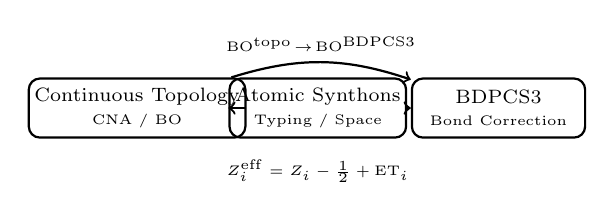
\begin{tikzpicture}[x=1cm,y=1cm,baseline=(current bounding box.center),scale=0.85]
\tikzstyle{box}=[draw,rounded corners,thick,align=center,inner sep=2pt,font=\scriptsize]
\node[box,minimum width=2.2cm,minimum height=0.75cm] (topo) at (0,0) {Continuous Topology\\\tiny CNA / BO};
\node[box,minimum width=2.2cm,minimum height=0.75cm] (syn) at (2.7,0) {Atomic Synthons\\\tiny Typing / Space};
\node[box,minimum width=2.2cm,minimum height=0.75cm] (bdp) at (5.4,0) {BDPCS3\\\tiny Bond Correction};

\draw[->,thick] (topo) -- (syn);
\draw[->,thick] (syn) -- (bdp);
\draw[->,thick] (topo) to[bend left=18] node[above,font=\tiny] {$\mathrm{BO}^{\mathrm{topo}}\!\to\!\mathrm{BO}^{\mathrm{BDPCS3}}$} (bdp);

\node[align=center,font=\tiny] at (2.7,-0.95) {$Z_i^{\mathrm{eff}}=Z_i-\frac{1}{2}+\mathrm{ET}_i$};
\end{tikzpicture}
\end{tocentry}

\end{document}
